\documentclass[10pt,twocolumn]{article}
	
\usepackage{myfontstyle}
\usepackage{mypackages}
\usepackage{mymacros}
\usepackage{mycommands}
\usepackage{url}

\begin{document}
\thispagestyle{fancy1}

%%% Title and Abstract------------------------
\twocolumn[
\begin{center}
	\hrule
	\vspace{3pt}
	% Title:
	{\sffamily\bfseries\Large
		Report for Laboratory Four: RLC Frequency Response 
	} \\
	{\color{gray}
		\vspace{3pt}
		\hrule
		\vspace{3pt}
	}
	{
		\hspace*{\fill}
		Austin Piper
		\hspace*{\fill}
		Alex Blakely
		\hspace*{\fill}
		Irfan Ahmed
		\hspace*{\fill}
%		Fourth Author    % uncomment these two lines if there's a fourth author
%		\hspace*{\fill}
	}\\
	\vspace{3pt}
	{\itshape
		\hspace*{\fill}
		Department of Mechanical Engineering, Saint Martin's University
		\hspace*{\fill} \\
		\hspace*{\fill}
		ME/EE 316---Mechatronics \& Measurements Laboratory
		\hspace*{\fill}
	}\\
	\vspace{3pt}
	{
		\hspace*{\fill}
		\today{} % today's date ... can type manually instead
		\hspace*{\fill}
	}
	\vspace{3pt}
	{\color{gray}\hrule}
%	\vspace{2pt}
\end{center}
% Abstract:
\begin{adjustwidth}{1.5in}{1.5in}
{\small
\noindent\textbf{Abstract.} \hspace{1em}
	In this lab exercise, we measured the steady-state response of the output voltage of an RLC circuit with a sinusoidal voltage source. We recorded the data by hand, and used MATLAB to plot the data and derive a model. Finally, we compared the analytic model to the experimental data.
}
\end{adjustwidth}
\vspace{9pt}
\hrule
\vspace{1\baselineskip}
]

%%% Body -------------------------


\section{Introduction} 
\label{sec:introduction}

An RLC circuit is a circuit that contains a resistor, and inductor, and a capacitor. This class of circuits is often used as oscillators. The characteristics of this type of circuit make it useful in signal filtering.

While, by definition, this kind of circuit can be any combination of these three circuit elements, in this experiment we put them together in Series. As \autoref{fig:diagram} shows, we assume that the voltage source (a signal generator) has a resistance Rs (which has a value of 50 \Omega).

\begin{figure}[bt]
	\centering
	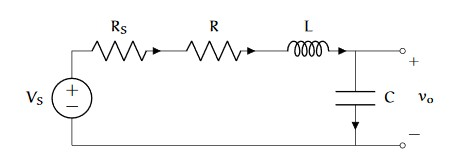
\includegraphics[width=.9\linewidth]{figures/RLCDiagram.JPG}
	\caption{The RLC Circuit}
	\label{fig:diagram}
\end{figure}

\section{Materials and Methods}

``This is like a cooking recipe. Include enough detail so that someone can repeat the experiment. It is important that the reader be able to interpret the results knowing the context in which they were obtained.

``The Materials and Methods section should be written in the past tense, since your experiments are completed at the time you are writing your paper.''

Here are some things you don't want to do in this section.

\begin{enumerate}
\item 
Don't simply copy and paste material from my description. 
\item 
Don't simply list the procedure in bullet points (although some lists are fine). I want a description in \emph{your} words.
\item
Don't use a figure from my description unless you properly cite it! A proper citation would be \citep[p.~32]{Picone2018}.
\end{enumerate}

\section{Results}
\label{sec:results}

\begin{figure}[bt]
	\centering
	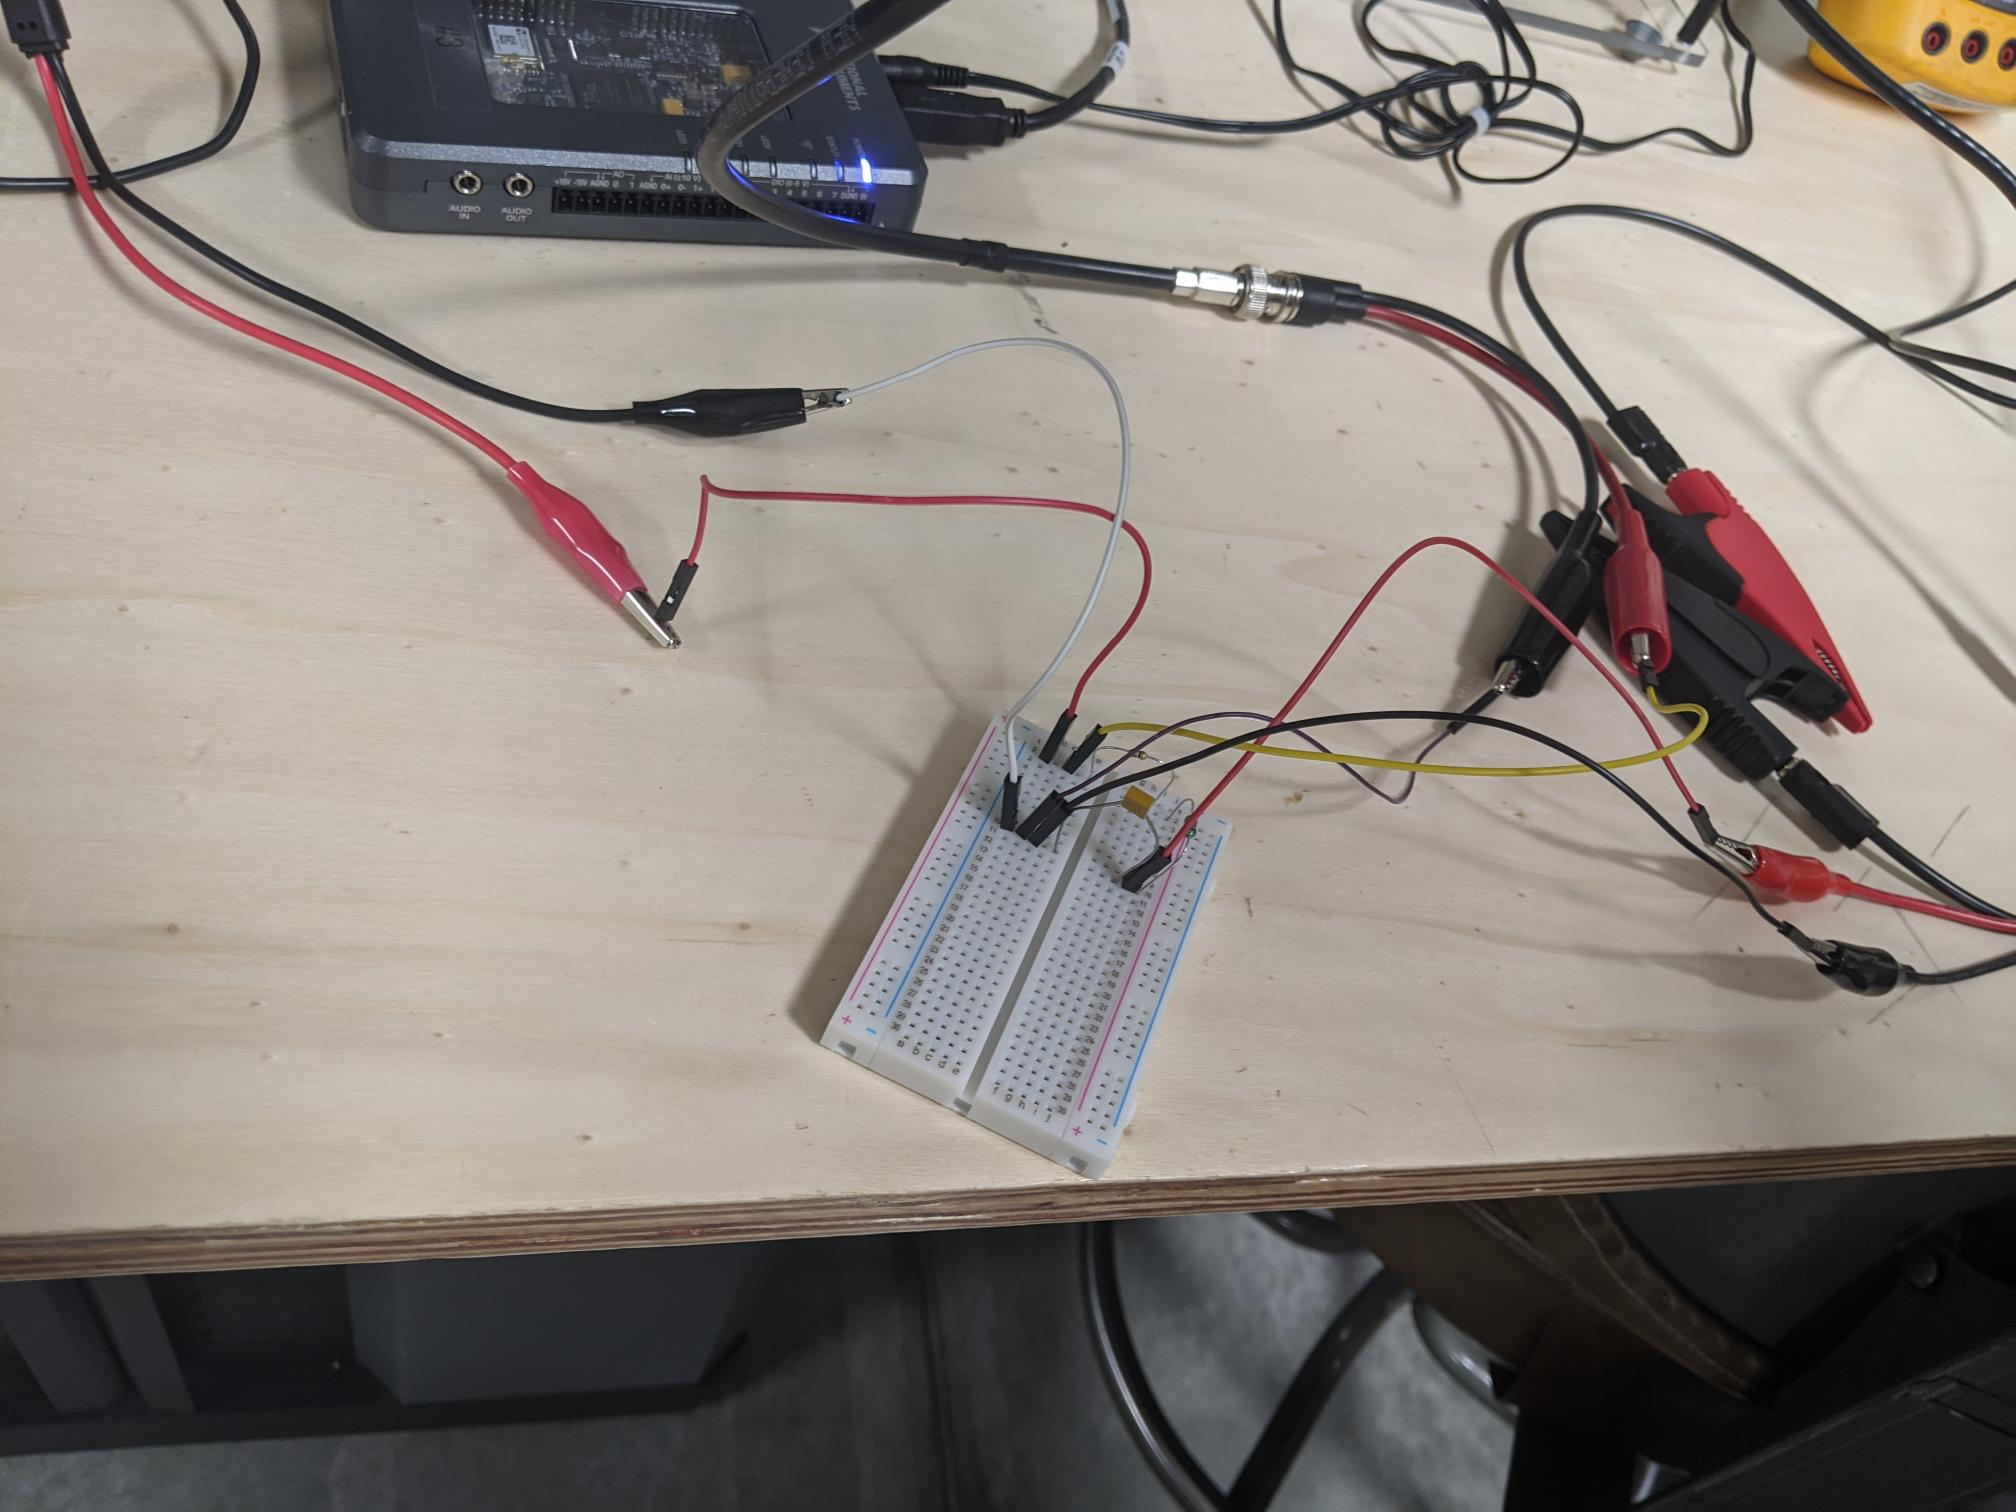
\includegraphics[width=.9\linewidth]{figures/RLCcircuit.PNG}
	\caption{RLC Circuit}
	\label{fig:diagram2}
\end{figure}
``To write the results section, use the figures and tables as a guide. Start by outlining, in point form, what you found, going slowly through each part of the figures. Then take the points and group them into paragraphs, and finally order the points within each paragraph. Present the data as fully as possible, including stuff that at the moment does not quite make sense.

``Verbs in the results section are usually in the past tense. Only established scientific knowledge is written about in the present tense, `the world is round,' for example. You cannot presume that your own data are part of the body of established scientific knowledge, and so when you describe your own results, use the past tense, `a band of 1.3 KB was seen,' for example. There are, however, exceptions to this general rule. It is acceptable to say, `Table 3 shows the sizes of the DNA fragments in our preparation.' It is also acceptable to say, `In a 1991 paper, Ebright and coworkers used PCR to mutagenize DNA.' \ldots

``Some readers begin by scanning the figures first. The figures, with the legends, should provide a self-explanatory overview of your data. Decide what the data show, then create figures which highlight the most important points of your paper.

``Tables are used to present repetitive data that is numerical. Graphs or illustrations, collectively called figures, are used to present numerical trends, raw data (like a picture of a gel), or a model that explains your work.

``When you prepare your figures and tables, keep in mind that it is significantly more expensive for journals to publish figures and tables than text, so try to present the data in a way that is worthy of such added expense.''

\section{Discussion}

``This is the section of the paper for you to show off your understanding of the data. You should summarize what you found. Explain how this relates to what others have found. Explain the implications.''

\section{Author Contributions}

You are required to describe each member's contributions to the laboratory exercise and report.






\end{document}  
